% !TEX root = task-3-20.tex
% Editable task bank. Append new BankTask blocks at the end of the document.
\documentclass[12pt,a4paper]{article}
\usepackage{physics-textbook}
\usepackage{graphicx,needspace}
\usetikzlibrary{decorations.pathmorphing}
\newif\ifShowSolutions
\ifdefined\TutorEdition
  \ShowSolutionstrue
\else
  \ShowSolutionsfalse % Change to \ShowSolutionstrue to display solutions.
\fi
\newcounter{banktask}
\newsavebox{\BankTaskBox}
\newcommand{\BankTaskContent}[3]{%
  \noindent\textbf{\thebanktask.}\quad #2\par
  \ifShowSolutions
    \Needspace{50mm}% Keep the solution heading with its opening text or diagram.
    #3\par
    \ifdefined\TutorEdition
      \ifcsname TutorSource#1\endcsname
        \nopagebreak\smallskip{\small\csname TutorSource#1\endcsname\par}%
      \fi
    \fi
  \fi
}
\newcommand{\BankTask}[3]{%
  \refstepcounter{banktask}\par\medskip
  \sbox{\BankTaskBox}{\begin{minipage}{\linewidth}%
    \BankTaskContent{#1}{#2}{#3}\end{minipage}}%
  \ifdim\dimexpr\ht\BankTaskBox+\dp\BankTaskBox\relax>\dimexpr\textheight-20mm\relax
    \Needspace{35mm}\BankTaskContent{#1}{#2}{#3}%
  \else
    \Needspace{\dimexpr\ht\BankTaskBox+\dp\BankTaskBox\relax}%
    \noindent\usebox{\BankTaskBox}\par
  \fi
  \medskip
}
\begin{document}
\BookSubsection{3.20}{Самоиндукция}


% Source 29735: https://phys-ege.sdamgia.ru/problem?id=29735
\BankTask{29735}{
\begin{center}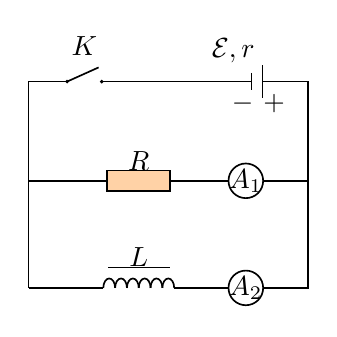
\begin{tikzpicture}[>=stealth,line width=.6pt]

\draw(0,0)--(0,2.62)--(.49,2.62) (.93,2.62)--(2.83,2.62) (2.97,2.62)--(3.55,2.62)--(3.55,0)--(2.98,0)
 (2.54,0)--(1.85,0) (.95,0)--(0,0) (0,1.36)--(1,1.36) (1.8,1.36)--(2.54,1.36) (2.98,1.36)--(3.55,1.36);
\draw(1.01,.26)--(1.8,.26);
\begin{scope}[shift={(0.71,2.62)},rotate=0]\draw(-.22,0)--(.18,.18);\fill(-.22,0)circle(.025) (.22,0)circle(.025);\node[above]at(0,.2){$K$};\end{scope}\begin{scope}[shift={(2.9,2.62)},rotate=180]\draw(-.07,-.21)--(-.07,.21) (.07,-.11)--(.07,.11);\end{scope}\node[above right] at (3.02,2.62) {$$};\node[above] at (2.6,2.73) {$\mathcal E,r$};\node[below] at (2.72,2.59) {$-$};\node[below] at (3.12,2.59) {$+$};\begin{scope}[shift={(1.4,1.36)},rotate=0]\draw[fill=orange!35] (-.4,-.13) rectangle (.4,.13);\end{scope}\node[above] at (1.4,1.36) {$R$};\begin{scope}[shift={(1.4,0)}]\foreach \x in {-.45,-.3,-.15,0,.15,.3}{\draw(\x,0)arc(180:0:.075 and .12);}\node[above] at (0,.15) {$L$};\end{scope}\draw (2.76,1.36)circle(.22) node {$A_1$};\draw (2.76,0)circle(.22) node {$A_2$};
\end{tikzpicture}\end{center}
 Резистор R и катушка индуктивности L с железным сердечником подключены к источнику тока, как показано на схеме. Первоначально ключ K замкнут, показания амперметров A$_{1}$ и A$_{2}$ равны, соответственно, $I_1=1 A$ и $I_2=0{,}1A.$ Что произойдет с величиной и направлением тока через резистор после размыкания ключа K? Ответ поясните, указав, какие явления и законы вы использовали для объяснения.
}{
\smallskip\noindent\textbf{Решение}\par
$1$.  При замкнутом ключе катушка и резистор соединены параллельно, токи в них будут иметь одинаковые направления. Исходя из схемы, токи текут от плюса к минусу, то есть справа налево. 
$2$.  После размыкания ключа в катушке будет наблюдаться явление самоиндукции, в результате чего в ней возникнет ЭДС самоиндукции $\mathcal E_{si}= - L \frac{\Delta I_2}{\Delta t} ,$ препятствующее уменьшению тока через катушку. Тогда ток через катушку будет иметь прежнее направление. 
$3$.  Так как источник тока отключен, а в цепи возникла ЭДС самоиндукции, то резистор будет подключен последовательно с катушкой. В результате ток через резистор изменит направление на противоположное, то есть будет течь слева направо. 
$4$.  Сразу после размыкания ключа через резистор будет течь такой же ток, как и через катушку. Следовательно, он станет равным I$_{2}$, то есть уменьшится от $1\,\text{А}$ до $0{,}1$ A.

Ответ: ток через резистор сразу после размыкания ключа будет течь вправо с силой тока $0{,}1\,\text{А}$.
}

% Source 29460: https://phys-ege.sdamgia.ru/problem?id=29460
\BankTask{29460}{
\begin{center}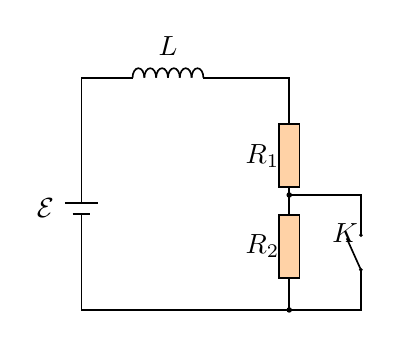
\begin{tikzpicture}[>=stealth,line width=.6pt]

\draw(0,.99)--(0,2.58)--(.65,2.58) (1.55,2.58)--(2.64,2.58)--(2.64,1.99)
 (2.64,1.19)--(2.64,.84) (2.64,.04)--(2.64,-.37)--(0,-.37)--(0,.85)
 (2.64,1.09)--(3.55,1.09)--(3.55,.58) (3.55,.14)--(3.55,-.37)--(2.64,-.37);
\fill(2.64,1.09)circle(.035) (2.64,-.37)circle(.035);
\begin{scope}[shift={(0,0.92)},rotate=-90]\draw(-.07,-.21)--(-.07,.21) (.07,-.11)--(.07,.11);\end{scope}\node[above right] at (0.12,0.92) {$$};\node[left]at(-.22,.92){$\mathcal E$};\begin{scope}[shift={(1.1,2.58)}]\foreach \x in {-.45,-.3,-.15,0,.15,.3}{\draw(\x,0)arc(180:0:.075 and .12);}\node[above] at (0,.15) {$L$};\end{scope}\begin{scope}[shift={(2.64,1.59)},rotate=90]\draw[fill=orange!35] (-.4,-.13) rectangle (.4,.13);\end{scope}\node[left] at (2.64,1.59) {$R_1$};\begin{scope}[shift={(2.64,0.44)},rotate=90]\draw[fill=orange!35] (-.4,-.13) rectangle (.4,.13);\end{scope}\node[left] at (2.64,0.44) {$R_2$};\begin{scope}[shift={(3.55,0.36)},rotate=90]\draw(-.22,0)--(.18,.18);\fill(-.22,0)circle(.025) (.22,0)circle(.025);\node[above]at(0,.2){$K$};\end{scope}
\end{tikzpicture}\end{center}
Катушка, обладающая индуктивностью L, соединена последовательно с источником постоянного тока с ЭДС $\mathcal{E}$ и резисторами R$_{1}$ и R$_{2}$, имеющими одинаковое сопротивление R$_{1}$ =  R$_{2}$  =  R, как показано на рисунке. В начальный момент ключ в цепи разомкнут. Как изменятся сила тока в цепи и напряжение на участке цепи, содержащем резистор R$_{1}$, после замыкания ключа? Ответ поясните, опираясь на законы электродинамики. Внутренним сопротивлением источника тока и сопротивлением катушки пренебречь.
}{
\smallskip\noindent\textbf{Решение}\par
$1$.  Сила тока определяется законом Ома для полной цепи: $IR_{\,\text{общ}}=\mathcal{E} + \mathcal E_{si},$ где I  — сила тока в цепи, $R_{\,\text{общ}}$  — сопротивление цепи, а $\mathcal E_{si}= - L \frac{\Delta I}{\Delta t}$  — ЭДС самоиндукции, возникающая только при изменении силы тока и препятствующая его изменению согласно правилу Ленца. 
$2$.  До замыкания ключа $R_{\,\text{общ}}=2R,$ сила тока через амперметр определяется законом Ома для замкнутой цепи: $I_1= \frac{\mathcal{E}}{2R} .$ 
$3$.  При замыкании ключа сопротивление цепи скачком уменьшается в $2$ раза, но ЭДС самоиндукции препятствует изменению силы тока через катушку. Поэтому сила тока через катушку при замыкании ключа не претерпевает скачка. 
$4$.  Постепенно ЭДС самоиндукции уменьшается до нуля, а сила тока через катушку плавно возрастает до стационарного значения: $I_2= \frac{\mathcal{E}}{R} ,$ в $2$ раза большего, чем начальное. 
$5$.  По закону Ома для участка цепи $U=IR_1$ увеличение тока через резистор R$_{1}$ приведет к увеличению напряжения на нем.
}

\end{document}
